% $Id: part1.tex,v 1.131 1999/05/16 14:16:33 bsmith Exp bsmith $ 

% --------------------------------------------------------------------
%
%                            PART 1
%
%   This introductory PETSc information is included in 
%   both manual.tex and intro.tex.
%
% --------------------------------------------------------------------

\label{sec:gettingstarted}

The Portable, Extensible Toolkit for Scientific Computation (PETSc)
has successfully demonstrated that the use of modern programming
paradigms can ease the development of large-scale scientific
application codes in Fortran, C, and C++.  Begun several years ago,
the software has evolved into a powerful set of tools for the
numerical solution of partial differential equations and related problems 
on high-performance computers.

PETSc consists of a variety of components (similar to classes in C++),
which are discussed in detail in Parts II and III of the users manual.
Each component manipulates a particular family of objects (for instance,
vectors) and the operations one would like to perform on the objects.
The objects and operations in PETSc are derived from our long 
experiences with scientific computation. Some of the PETSc modules deal with 
\begin{itemize} 
\item index sets, including permutations, for indexing into vectors, renumbering, etc;
\item vectors;
\item matrices (both sparse and dense);
\item distributed arrays (useful for parallelizing regular grid-based 
      problems);
\item Krylov subspace methods;
\item preconditioners;
\item nonlinear solvers;
\item unconstrained minimization;
\item timesteppers for solving time-dependent (nonlinear) PDEs; and
\item graphics devices.
\end{itemize}
Each of these components consists of an abstract interface 
(simply a set of calling sequences) and one or more implementations 
using particular data structures. Thus, PETSc provides clean and 
effective codes for the various phases of solving PDEs, with a uniform 
approach for each class of problems.  This design
enables easy comparison and use of different algorithms (for example,
to experiment with different Krylov subspace methods, preconditioners,
or truncated Newton methods).
Hence, PETSc provides a rich environment for modeling scientific
applications as well as for rapid algorithm design and prototyping.

The components enable easy customization and extension of both algorithms
and implementations.  This approach promotes code reuse and
flexibility, and separates the issues of parallelism from the choice
of algorithms.  The PETSc infrastructure creates a
foundation for building large-scale applications.

It is useful to consider the interrelationships among different
pieces of PETSc 2.0.  Figure \ref{fig:1} is a diagram of some 
of the components of PETSc; Figure \ref{fig:2} presents
several of the individual components in more detail.
These figures illustrate the library's hierarchical organization,
which enables users to employ the level of abstraction that is most 
appropriate for a particular problem.  
\begin{figure}[hbt]
\centerline{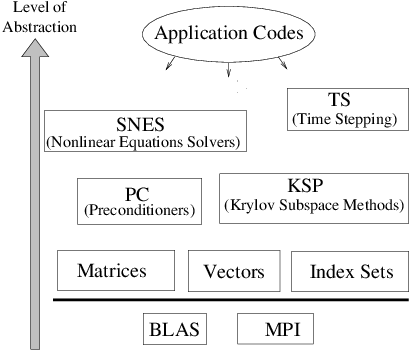
\psfig{file=petscwww.ps,angle=270,height=3.4in}}
% \centerline{\psfig{file=petsc_pt.eps,angle=0,height=4in,width=5in}}
\caption{Organization of the PETSc Library}
\label{fig:1}
\end{figure}

\begin{figure}[hbt]
\centerline{\psfig{file=zoom_ls.ps,angle=270,height=3.4in}}
\caption{Numerical Components of PETSc}
\label{fig:2}
\end{figure}

\section{Suggested Reading}

The manual is
divided into three parts:
\begin{itemize}
\item Part I - Introduction to PETSc
\item Part II - Programming with PETSc
\item Part III - Additional Information
\end{itemize}

Part I describes
the basic procedure for using the PETSc library and presents two
simple examples of solving linear systems with PETSc.  This section
conveys the typical style used throughout the library and enables the
application programmer to begin using the software immediately.
Part I is also distributed separately for individuals interested in an 
overview of the PETSc software, excluding the details of library usage.
Readers of this separate distribution of Part I should note that all
references within the text to particular chapters and sections 
indicate locations in the complete users manual.

Part II explains in detail the use of the various PETSc components,
such as vectors, matrices, index sets, linear and nonlinear
solvers, and graphics.  Part III describes a variety of useful
information, including profiling, the options database, viewers, error
handling, makefiles, and some details of
PETSc design.

\nocite{efficient}

The {\em PETSc 2.0 Users Manual} documents {\em all} of PETSc 2.0; thus,
it can be rather intimidating for new users. We recommend that one initially
read the entire document before proceeding with serious use of PETSc,
but bear in mind that PETSc can be used efficiently
before one understands all of the material presented here. 

\medskip \medskip

Within the PETSc distribution, the directory
{\tt \$\{PETSC\_DIR\}/docs} contains all documentation.
Manual pages for all PETSc functions can be
accessed on line at
\begin{verbatim}
  ${PETSC_DIR}/docs/manualpages/index.html
\end{verbatim}
The manual pages
provide hyperlinked indices (organized by
both concepts and routine names) to the tutorial examples and enable
easy movement among related topics.  

Emacs users may find the
{\em etags} option to be extremely useful for exploring the PETSc
source code.  Details of this feature are provided in
Section~\ref{sec:emacs}. 

The file {\tt manual.ps} contains the PostScript form of
the {\em PETSc 2.0 Users Manual} in its entirety, while {\tt intro.ps} 
includes only the introductory segment, Part I.  \sindex{installing PETSc} 
The file {\tt Installation} contains detailed instructions for
installing PETSc. The complete PETSc distribution, users
manual, manual pages, and additional information are also available via
the PETSc home page at
{\tt http://www.mcs.anl.gov/petsc}.  The PETSc home page also
contains details regarding installation, new features and changes in recent
versions of PETSc, machines that we currently support, a
troubleshooting guide, and a FAQ list for frequently asked questions.

\medskip \medskip

{\bf Note to Fortran Programmers}: In most of the  
manual, the examples and calling sequences are given for the C/C++
family of programming languages.  We follow this convention because we
recommend that PETSc applications be coded in C or C++.
However, pure Fortran programmers can use most of the
functionality of PETSc from Fortran, with only minor differences in
the user interface.  Chapter \ref{ch:fortran} provides a discussion of the
differences between using PETSc from Fortran and C, as well as several
complete Fortran examples.  This chapter also introduces some
routines that support direct use of Fortran90 pointers.

%-----------------------------------------------------------------------------
\section{Running PETSc Programs}
\label{sec:running}

Before using PETSc, the user must first set the environmental variable
{\tt PETSC\_DIR}, \findex{PETSC_DIR} indicating the full path of the PETSc home
directory.  For example, under the UNIX C shell a command of the form
\begin{verbatim}
   setenv PETSC_DIR $HOME/petsc
\end{verbatim}
 can be placed in the user's {\tt
.cshrc} file.  In addition, the user must set the environmental
variable {\tt PETSC\_ARCH} to specify the architecture (e.g., rs6000,
sun4, solaris, etc.)  on which PETSc is being used.  The utility {\tt
\$\{PETSC\_DIR\}/bin/petscarch} can be used for this purpose.  For example,
\begin{verbatim}
   setenv PETSC_ARCH `$PETSC_DIR/bin/petscarch`
\end{verbatim}
can be placed in a {\tt .cshrc} file.  Thus, even if several machines of different
types share the same filesystem, {\tt PETSC\_ARCH} will be set correctly
when logging into any of them. 

All PETSc programs use the MPI (Message Passing Interface) standard
for message-passing communication \cite{MPI-final}.  Thus, to execute
PETSc programs, users must know the procedure for beginning MPI jobs
on their selected computer system(s).  For instance, when using the
MPICH implementation of MPI \cite{mpich-web-page} and many others, the following
command initiates a program that uses eight processors:
\findex{mpirun} \sindex{running PETSc programs} 
\begin{verbatim}
   mpirun -np 8 petsc_program_name petsc_options
\end{verbatim}


All PETSc 2.0-compliant programs support the use of the {\tt -h}
\findex{-h} or {\tt -help} option as well as the {\tt -v} \findex{-v}
or {\tt -version} option. 


Certain options are supported by all PETSc programs.  We list a few 
particularly useful ones below; a complete list can be obtained by 
running any PETSc program with the option {\tt -help}.
\begin{itemize}
\item {\tt -log\_summary} - summarize the program's performance
\item {\tt -fp\_trap} - stop on floating-point exceptions; \findex{-fp_trap}
      for example divide by zero
\item {\tt -trdump} - enable memory tracing; dump list of unfreed memory 
      at conclusion \findex{-trdump} of the run
\item {\tt -trmalloc} - enable memory tracing (by default this is 
      activated for the debugging versions of PETSc)
\item {\tt -start\_in\_debugger [noxterm,gdb,dbx,xxgdb] [-display name]} 
     - start all processes in debugger \findex{-start_in_debugger} \sindex{debugger}
\item {\tt -on\_error\_attach\_debugger \findex{-on_error_attach_debugger} [noxterm,gdb,dbx,xxgdb]
      [-display name]} - start debugger only on encountering an error
\end{itemize}
See Section \ref{sec:debugging} for more information on debugging PETSc programs.

%-----------------------------------------------------------------------------
\section{Writing PETSc Programs}
\label{sec:writing}

Most PETSc programs begin with a call to \findex{PetscInitialize()}
\begin{verbatim}
   ierr = PetscInitialize(int *argc,char ***argv,char *file_name,char *help_message);
\end{verbatim} 
which initializes PETSc and MPI.  The arguments {\tt argc} and 
{\tt argv} are the command line arguments delivered in all C and C++
programs. \sindex{command line arguments} The argument {\tt file\_name}
optionally indicates an alternative name for the PETSc options file,
{\tt .petscrc}, which resides by default in the user's home directory.
Section \ref{sec:options} provides details regarding
this file and the PETSc options database, which can be used for runtime
customization. The final argument, {\tt help\_message}, is an optional
character string that will be printed if the program is run with the
{\tt -help} option.  In Fortran the initialization command has the form
\begin{verbatim}
   call PetscInitialize(character file_name,integer ierr)
\end{verbatim} 
{\tt PetscInitialize()} automatically calls {\tt MPI\_Init()} if MPI
has not been not previously initialized. In certain \findex{MPI_Init()}
circumstances in which MPI needs to be initialized directly (or is
initialized by some other library), the user should first call 
{\tt MPI\_Init()} (or have the other library do it), and then call
{\tt PetscInitialize()}.
By default, {\tt PetscInitialize()} sets the PETSc ``world''
communicator, given by {\tt PETSC\_COMM\_WORLD}, to {\tt MPI\_COMM\_WORLD}.
\findex{PETSC_COMM_WORLD}

For those not familar with MPI, a {\em communicator} is a way of
indicating a collection of processors that will be involved together
in a calculation or communication. Communicators have the variable type
{\tt MPI\_Comm}. In most cases users can employ the communicator {\tt
PETSC\_COMM\_WORLD} to indicate all processes in a given run and {\tt
PETSC\_COMM\_SELF} to indicate a single process. MPI provides routines
for generating new communicators consisting of subsets of processors,
though most users rarely need to use these. The book {\em Using MPI},
by Lusk, Gropp, and Skjellum \cite{using-mpi} provides an excellent
introduction to the concepts in MPI. Note that PETSc users need not
program much message passing directly with MPI, but they must be
familar with the basic concepts of message passing and distributed
memory computing.

Users who wish to employ PETSc routines on only a subset
of processors within a larger parallel job, or who wish to use a
``master'' process to coordinate the work of ``slave'' PETSc
processes, should specify an alternative communicator for {\tt
PETSC\_COMM\_WORLD} by calling \findex{PetscSetCommWorld}
\sindex{communicator}
\begin{verbatim}
   ierr = PetscSetCommWorld(MPI_Comm comm);
\end{verbatim}
{\em before} calling {\tt PetscInitialize()}, but, obviously, after
calling {\tt MPI\_Init()}. {\tt PetscSetCommWorld()} can be called
at most once per process. Most users will never need to use the routine
{\tt PetscSetCommWorld()}.

As illustrated by the {\tt PetscInitialize()} statements above,
PETSc~2.0 routines return an integer indicating whether an error has
occurred during the call.  The error code is set to be nonzero if an
error has been detected; otherwise, it is zero.  For the C/C++
interface, the error variable is the routine's return value, while for
the Fortran version, each PETSc routine has as its final argument an
integer error variable.  Error tracebacks are discussed in the following
section.

All PETSc programs should call {\tt PetscFinalize()} \findex{PetscFinalize()}
as their final (or nearly final) statement, as given below in the C/C++
and Fortran formats, respectively:
\begin{verbatim}
   ierr = PetscFinalize();
   call PetscFinalize(ierr)
\end{verbatim}
This routine handles options to be called at the conclusion of
the program, and calls {\tt MPI\_Finalize()} \findex{MPI_Finalize()}
if {\tt PetscInitialize()}
began MPI. If MPI was initiated externally from PETSc (by either
the user or another software package), the user is
responsible for calling {\tt MPI\_Finalize()}. 

\section{Simple PETSc Examples}

\label{sec:simple}

To help the user start using PETSc immediately, we begin with a simple
uniprocessor example in Figure~\ref{fig:example1} that solves the
one-dimensional Laplacian problem with finite differences.  This
sequential code, which can be found in 
{\tt \$\{PETSC\_DIR\}/src/sles/examples/tutorials/ex1.c},
illustrates the solution of a linear system with SLES, the 
interface to the preconditioners, Krylov subspace methods, and direct
linear solvers of PETSc.  Following the code we highlight a few of the most important
parts of this example.  

\begin{figure}[H]
{\footnotesize
\fileinclude{../../../src/sles/examples/tutorials/ex1.c}
}
\caption{Example of Uniprocessor PETSc Code}
\label{fig:example1}
\end{figure}

\subsection*{Include Files}

The C/C++ include files for PETSc should be used via statements such as
\begin{verbatim}
   #include "sles.h"
\end{verbatim}
where {\tt sles.h} is the include file for the SLES component.
Each PETSc program must specify an
include file that corresponds to the highest level PETSc objects
needed within the program; all of the required lower level include
files are automatically included within the higher level files.  For
example, {\tt sles.h} includes {\tt mat.h} (matrices),
{\tt vector.h} (vectors), and {\tt petsc.h} (base PETSc file).  
The PETSc include files are located in the directory 
{\tt \$\{PETSC\_DIR\}/include}.  See Section \ref{sec:fortran_includes}
for a discussion of PETSc include files in Fortran programs.

\subsection*{The Options Database}

As shown in Figure~\ref{fig:example1}, the user can input control data
at run time using the options database. In this example the command
{\tt OptionsGetInt(PETSC\_NULL,"-n",\&n,\&flg);} checks whether the user has
provided a command line option to set the value of {\tt n}, the
problem dimension.  If so, the variable {\tt n} is set accordingly;
otherwise, {\tt n} remains unchanged. A complete description of the
options database may be found in Section \ref{sec:options}.

\subsection*{Vectors}
\label{sec:vecintro}

One creates a new parallel or 
sequential vector, {\tt x}, of global dimension {\tt M} with the 
command \findex{VecCreate()} \sindex{vectors}
\begin{verbatim}
   ierr = VecCreate(MPI_Comm comm,int m,int M,Vec *x);
\end{verbatim}
where {\tt comm} denotes the MPI communicator. The type of storage
for the vector may be set with either calls to 
{\tt VecSetType()} or {\tt VecSetFromOptions()}. \findex{VecSetType()} \findex{VecSetFromOptions}
Additional vectors of the same type can be formed with
\findex{VecDuplicate()}
\begin{verbatim}
   ierr = VecDuplicate(Vec old,Vec *new);
\end{verbatim}
The commands \findex{VecSet()} \findex{VecSetValues()}
\begin{verbatim}
   ierr = VecSet(Scalar *value,Vec x);
   ierr = VecSetValues(Vec x,int n,int *indices,Scalar *values,INSERT_VALUES);
\end{verbatim}
respectively set all the components of a vector to a particular scalar
value and assign a different value to each component.  More
detailed information about PETSc vectors, including their basic
operations, scattering/gathering, index sets, and distributed arrays, is
discussed in Chapter~\ref{chapter:vectors}.

\findex{Scalar} \sindex{complex numbers}
Note the use of the PETSc variable type {\tt Scalar} in this example.
The {\tt Scalar} is simply defined to be {\tt double} in C/C++
(or correspondingly {\tt double precision} in Fortran) for versions of
PETSc that have {\em not} been compiled for use with complex numbers.
The {\tt Scalar} data type enables
identical code to be used when the PETSc libraries have been compiled
for use with complex numbers.  Section~\ref{sec:complex} discusses the
use of complex numbers in PETSc programs.

\subsection*{Matrices}
\label{sec:matintro}

Usage of PETSc matrices and vectors is similar. \sindex{matrices} 
The user can create a new parallel or sequential matrix, {\tt A}, which
has {\tt M} global rows and {\tt N} global columns, with the routine
\findex{MatCreate()}
\begin{verbatim}
   ierr = MatCreate(MPI_Comm comm,int m,int n,int M,int N,Mat *A);
\end{verbatim}
where the matrix format can be specified at runtime.  The user could
alternatively specify each processes' number of local rows and columns
using {\tt m} and {\tt n}.
Values can then be set with the command
\begin{verbatim}
   ierr = MatSetValues(Mat A,int m,int *im,int n,int *in,Scalar *values,INSERT_VALUES);
\end{verbatim}
After \findex{MatSetValues()} all elements have been inserted into the
matrix, it must be processed with the pair of commands
\findex{MatAssemblyBegin()} \findex{MatAssemblyEnd()}
\begin{verbatim}
   ierr = MatAssemblyBegin(Mat A,MAT_FINAL_ASSEMBLY);
   ierr = MatAssemblyEnd(Mat A,MAT_FINAL_ASSEMBLY);
\end{verbatim}
Chapter~\ref{chapter:matrices} discusses various matrix formats as
well as the details of some basic matrix manipulation routines.

\subsection*{Linear Solvers}

After creating the matrix and vectors that define a linear system,
{\tt Ax = b}, the user can then use SLES to solve the system 
with the following sequence of commands: 
\findex{SLESCreate()} \findex{SLESSetOperators()}
\findex{SLESSetFromOptions()} \findex{SLESSolve()} \findex{SLESDestroy()}
\begin{verbatim}
   ierr = SLESCreate(MPI_Comm comm,SLES *sles); 
   ierr = SLESSetOperators(SLES sles,Mat A,Mat PrecA,MatStructure flag);
   ierr = SLESSetFromOptions(SLES sles);
   ierr = SLESSolve(SLES sles,Vec b,Vec x,int *its);
   ierr = SLESDestroy(SLES sles);
\end{verbatim}
The user first creates the SLES context and sets the operators
associated with the system (linear system matrix and optionally different
preconditioning matrix).  The user then sets various options for
customized solution, solves the linear system, and finally destroys
the SLES context.  We emphasize the command {\tt SLESSetFromOptions()}, 
which enables the user to customize the linear solution
method at runtime by using the options database, which is discussed in
Section~\ref{sec:options}. Through this database, the user not only
can select an iterative method and preconditioner, but also can prescribe
the convergence tolerance, set various monitoring routines, etc.
(see, e.g., Figure~\ref{fig:exprof}).

Chapter~\ref{ch:sles} describes in detail the SLES package, including
the PC and KSP components for preconditioners and Krylov subspace methods.

\subsection*{Error Checking}

All PETSc 2.0 routines return an integer indicating whether an error
has occurred during the call.  The PETSc macro {\tt CHKERRQ(ierr)}
checks the value of {\tt ierr} and calls the PETSc 2.0 error handler
upon error detection.  {\tt CHKERRQ(ierr)} should be used in all
subroutines to enable a complete error traceback.  A variant of this
macro, {\tt CHKERRA(ierr)}, should be used in the main program to
enable correct termination of all processes when an error is
encountered.  In Figure~\ref{fig:traceback} we indicate a
traceback generated by error detection within a sample PETSc
program. The error occurred on line 858 of the file {\tt
\$\{PETSC\_DIR\}/src/mat/impls/aij/seq/aij.c} and was caused by trying to allocate too
large an array in memory. The routine was called in the program 
{\tt ex3.c} on line 49.  See Section \ref{sec:fortran_errors} for
details regarding error checking when using the PETSc Fortran interface.

\begin{figure}[H]
{\small
\begin{verbatim}
   eagle>mpirun -np 1 ex3 -m 10000
   [0]PETSC ERROR: MatCreateSeqAIJ() line 1673 in src/mat/impls/aij/seq/aij.c
   [0]PETSC ERROR:   Out of memory. This could be due to allocating
   [0]PETSC ERROR:   too large an object or bleeding by not properly
   [0]PETSC ERROR:   destroying unneeded objects.
   [0]PETSC ERROR:   Try running with -trdump for more information. 
   [0]PETSC ERROR: MatCreate() line 99 in src/mat/utils/gcreate.c  
   [0]PETSC ERROR: main() line 71 in src/sles/examples/tutorials/ex3.c  
   [0] MPI Abort by user Aborting program !
   [0] Aborting program!
   p0_28969:  p4_error: : 1
\end{verbatim}
}
\nobreak
\caption{Example of Error Traceback}
\label{fig:traceback}
\end{figure}

When running the debug (BOPT=g compiled) version of the PETSc libraries, it
does a great deal of checking for memory corruption (writing outside of 
array bounds etc). The macros {\tt CHKMEMQ} and {\tt CHKMEMA} can be called 
anywhere in the code to check the current status of the memory for corruption.
By putting several (or many) of these macros into your code you can usually 
easily track down in what small segment of your code the corruption has occured.

\subsection*{Parallel Programming}

Since PETSc uses the message-passing model for
parallel programming and employs MPI for all interprocessor
communication, the user is free to employ MPI routines as needed
throughout an application code.  However, by default the user is
shielded from many of the details of message passing within PETSc,
since these are hidden within parallel objects, such as vectors,
matrices, and solvers.  In addition, PETSc provides tools such as
generalized vector scatters/gathers and distributed arrays to assist
in the management of parallel data.

\sindex{collective operations}
Recall that the user must specify a communicator upon creation of any
PETSc object (such as a vector, matrix, or solver) to indicate the
processors over which the object is to be distributed.  For example,
as mentioned above, some commands for matrix, vector, and linear solver
creation are:
\begin{verbatim}
   ierr = MatCreate(MPI_Comm comm,int M,int N,Mat *A);
   ierr = VecCreate(MPI_Comm comm,int m,int M,Vec *x);
   ierr = SLESCreate(MPI_Comm comm,SLES *sles); 
\end{verbatim}
The creation routines are collective over all processors in the
communicator; thus, all processors in the communicator {\em must}
call the creation routine.  In addition, if a sequence of
collective routines is being used, they {\em must} be called
in the same order on each processor.

The next example, given in Figure~\ref{fig:example2}, illustrates the
solution of a linear system in parallel.  This code, corresponding to
{\tt \$\{PETSC\_DIR\}/src/sles/examples/tutorials/ex2.c}, handles the
two-dimensional Laplacian discretized with finite differences, where
the linear system is again solved with SLES.  The code performs the
same tasks as the sequential version within Figure~\ref{fig:example1}.
Note that the user interface for initiating the program, creating
vectors and matrices, and solving the linear system is {\em exactly}
the same for the uniprocessor and multiprocessor examples.  The
primary difference between the examples in Figures \ref{fig:example1}
and \ref{fig:example2} is that each processor forms only its local
part of the matrix and vectors in the parallel case.

\begin{figure}[H]
{\footnotesize
\fileinclude{../../../src/sles/examples/tutorials/ex2.c}
}
\nobreak
\caption{Example of Multiprocessor PETSc Code}
\label{fig:example2}
\end{figure}

\subsection*{Compiling and Running Programs}

Figure~\ref{fig:exrun} illustrates compiling and running a PETSc program
using MPICH.  Note that different sites may have slightly different
library and compiler names.  See Chapter \ref{ch:makefiles}
for a discussion about compiling PETSc programs.
Users who are experiencing difficulties linking PETSc programs should 
refer to the troubleshooting guide via the PETSc WWW home page 
{\tt http://www.mcs.anl.gov/petsc} or
given in the file {\tt \$\{PETSC\_DIR\}/docs/troubleshooting.html}.

\begin{figure}[H]
{\small
\begin{verbatim}
   eagle> make BOPT=g ex2
   gcc -DPETSC_ARCH_sun4 -pipe -c  -I../../../  -I../../..//include   
       -I/usr/local/mpi/include  -I../../..//src -g 
       -DPETSC_USE_DEBUG -DPETSC_MALLOC -DPETSC_USE_LOG ex1.c
   gcc -g -DPETSC_USE_DEBUG -DPETSC_MALLOC -DPETSC_USE_LOG -o ex1 ex1.o 
      /home/bsmith/petsc/lib/libg/sun4/libpetscsles.a 
      -L/home/bsmith/petsc/lib/libg/sun4 -lpetscstencil -lpetscgrid  -lpetscsles 
      -lpetscmat  -lpetscvec -lpetscsys -lpetscdraw  
      /usr/local/lapack/lib/lapack.a /usr/local/lapack/lib/blas.a 
      /usr/lang/SC1.0.1/libF77.a -lm /usr/lang/SC1.0.1/libm.a -lX11 
      /usr/local/mpi/lib/sun4/ch_p4/libmpi.a
      /usr/lib/debug/malloc.o /usr/lib/debug/mallocmap.o  
      /usr/lang/SC1.0.1/libF77.a -lm /usr/lang/SC1.0.1/libm.a -lm
   rm -f ex1.o
   eagle> mpirun -np 1 ex2
   Norm of error 3.6618e-05 iterations 7
   eagle>
   eagle> mpirun -np 2 ex2
   Norm of error 5.34462e-05 iterations 9
\end{verbatim}
}
\nobreak
\caption{Running a PETSc Program}
\label{fig:exrun}
\end{figure}

As shown in Figure \ref{fig:exprof}, the option {\tt
-log\_summary} activates printing of a performance summary, including
times, floating point operation (flop) rates, and message-passing
activity.  Chapter~\ref{ch:profiling}
provides details about profiling, including interpretation of the
output data within Figure~\ref{fig:exprof}.  This particular example involves the solution of a linear
system on one processor using GMRES and ILU.  The low floating point
operation (flop) rates in this example are due to the fact that the
code solved a tiny system.  We include this example merely to
demonstrate the ease of extracting performance information.

\begin{figure}[H]
{\footnotesize
\begin{verbatim}
eagle> mpirun -np 1 ex1 -n 1000 -pc_type ilu -ksp_type gmres -ksp_rtol 1.e-7 -log_summary
-------------------------------- PETSc Performance Summary: --------------------------------------

ex1 on a sun4 named merlin.mcs.anl.gov with 1 processor, by curfman Wed Aug  7 17:24:27 1996

                         Max         Min        Avg        Total 
Time (sec):           1.150e-01      1.0   1.150e-01
Objects:              1.900e+01      1.0   1.900e+01
Flops:                3.998e+04      1.0   3.998e+04  3.998e+04
Flops/sec:            3.475e+05      1.0              3.475e+05
MPI Messages:         0.000e+00      0.0   0.000e+00  0.000e+00
MPI Messages:         0.000e+00      0.0   0.000e+00  0.000e+00 (lengths)
MPI Reductions:       0.000e+00      0.0

--------------------------------------------------------------------------------------------------
Phase             Count      Time (sec)       Flops/sec                             -- Global --    
                            Max     Ratio    Max    Ratio   Mess  Avg len  Reduct  %T %F %M %L %R   
--------------------------------------------------------------------------------------------------
MatMult               2  2.553e-03    1.0  3.9e+06    1.0  0.0e+00 0.0e+00 0.0e+00  2 25  0  0  0
MatAssemblyBegin      1  2.193e-05    1.0  0.0e+00    0.0  0.0e+00 0.0e+00 0.0e+00  0  0  0  0  0
MatAssemblyEnd        1  5.004e-03    1.0  0.0e+00    0.0  0.0e+00 0.0e+00 0.0e+00  4  0  0  0  0
MatGetReordering      1  3.004e-03    1.0  0.0e+00    0.0  0.0e+00 0.0e+00 0.0e+00  3  0  0  0  0
MatILUFctrSymbol      1  5.719e-03    1.0  0.0e+00    0.0  0.0e+00 0.0e+00 0.0e+00  5  0  0  0  0
MatLUFactorNumer      1  1.092e-02    1.0  2.7e+05    1.0  0.0e+00 0.0e+00 0.0e+00  9  7  0  0  0
MatSolve              2  4.193e-03    1.0  2.4e+06    1.0  0.0e+00 0.0e+00 0.0e+00  4 25  0  0  0
MatSetValues       1000  2.461e-02    1.0  0.0e+00    0.0  0.0e+00 0.0e+00 0.0e+00 21  0  0  0  0
VecDot                1  2.060e-04    1.0  9.7e+06    1.0  0.0e+00 0.0e+00 0.0e+00  0  5  0  0  0
VecNorm               3  5.870e-04    1.0  1.0e+07    1.0  0.0e+00 0.0e+00 0.0e+00  1 15  0  0  0
VecScale              1  1.640e-04    1.0  6.1e+06    1.0  0.0e+00 0.0e+00 0.0e+00  0  3  0  0  0
VecCopy               1  3.101e-04    1.0  0.0e+00    0.0  0.0e+00 0.0e+00 0.0e+00  0  0  0  0  0
VecSet                3  5.029e-04    1.0  0.0e+00    0.0  0.0e+00 0.0e+00 0.0e+00  0  0  0  0  0
VecAXPY               3  8.690e-04    1.0  6.9e+06    1.0  0.0e+00 0.0e+00 0.0e+00  1 15  0  0  0
VecMAXPY              1  2.550e-04    1.0  7.8e+06    1.0  0.0e+00 0.0e+00 0.0e+00  0  5  0  0  0
SLESSolve             1  1.288e-02    1.0  2.2e+06    1.0  0.0e+00 0.0e+00 0.0e+00 11 70  0  0  0
SLESSetUp             1  2.669e-02    1.0  1.1e+05    1.0  0.0e+00 0.0e+00 0.0e+00 23  7  0  0  0
KSPGMRESOrthog        1  1.151e-03    1.0  3.5e+06    1.0  0.0e+00 0.0e+00 0.0e+00  1 10  0  0  0
PCSetUp               1  2.024e-02    1.0  1.5e+05    1.0  0.0e+00 0.0e+00 0.0e+00 18  7  0  0  0
PCApply               2  4.474e-03    1.0  2.2e+06    1.0  0.0e+00 0.0e+00 0.0e+00  4 25  0  0  0
-------------------------------------------------------------------------------------------------

Memory usage is given in bytes:

Object Type      Creations   Destructions   Memory  Descendants' Mem.
Index set             3              3      12420     0
Vector                8              8      65728     0
Matrix                2              2     184924     4140
Krylov Solver         1              1      16892     41080
Preconditioner        1              1          0     64872
SLES                  1              1          0     122844

\end{verbatim}
}
\nobreak
\caption{Running a PETSc Program with Profiling}
\label{fig:exprof}
\end{figure}

\subsection*{Writing Application Codes with PETSc}

The examples throughout the library demonstrate thesoftware usage
and can serve as templates for developing
custom applications.  We suggest that new PETSc
users examine programs in the directories 
\begin{verbatim}
  ${PETSC_DIR}/src/<component>/examples/tutorials,
\end{verbatim}
where {\tt <component>}
denotes any of the PETSc components (listed in the following
section), such as {\tt snes} or {\tt sles}.  
The HTML version of the manual pages located at
\begin{verbatim}
   ${PETSC_DIR}/docs/manualpages/index.html or 
   http://www.mcs.anl.gov/petsc/docs/manualpages/index.html
\end{verbatim}
provides indices (organized by both routine names and concepts) to the tutorial examples.

To write a new application program using PETSc, we suggest the
following procedure:
\begin{enumerate}
\item Install and test PETSc according to the instructions in 
      {\tt \$\{PETSC\_DIR\}/docs/installation.html}.
\item Copy one of the many PETSc examples in the component directory
      that corresponds to the class of problem of interest (e.g.,
      for linear solvers, see {\tt \$\{PETSC\_DIR\}/src/sles/examples/tutorials}).
\item Copy the corresponding makefile within the example directory;
      compile and run the example program.
\item Use the example program as a starting point for developing a custom code.
\end{enumerate}

%---------------------------------------------------------------------

\section{Referencing PETSc}

When referencing PETSc in a publication please cite the following:
\begin{verbatim}
@Unpublished{petsc-home-page,
   Author = "Satish Balay and William D. Gropp and Lois Curfman  McInnes and Barry F. Smith",
   Title  = "{PETSc} home page",
   Note   = <a href="http://www.mcs.anl.gov/petsc">"http://www.mcs.anl.gov/petsc",
   Year   = "1998"}

@TechReport{petsc-manual,
   Author      = "Satish Balay and William D. Gropp and Lois Curfman McInnes and Barry F. Smith",
   Title       = "{PETSc} 2.0 Users Manual",
   Number      = "ANL-95/11 - Revision 2.0.24",
   Institution = "Argonne National Laboratory",
   Year        = "1999"}

@InProceedings{petsc-efficient,
   Author    = "Satish Balay and William D. Gropp and Lois Curfman McInnes and Barry F. Smith",
   Title     = "Efficienct Management of Parallelism in Object Oriented Numerical Software Libraries",
   Booktitle = "Modern Software Tools in Scientific Computing",
   Editor    = "E. Arge and A. M. Bruaset and H. P. Langtangen",
   Pages     = "163--202",
   Publisher = "Birkhauser Press",
   Year      = "1997"}
\end{verbatim}


%---------------------------------------------------------------------

\section{Directory Structure}

We conclude this introduction with an overview of the
organization of the PETSc software.  
The root directory of PETSc contains the following directories:
% As shown in Figure~\ref{fig:directories}, the root directory of PETSc contains the following directories:

\begin{itemize}
\item {\tt docs} - All documentation for PETSc. The files {\tt manual.ps}
                   and {\tt manual.html} contain the users manual in
                   PostScript and HTML formats, respectively. Includes
                   the subdirectory
 \subitem - {\tt manualpages} (on-line manual pages).
\item {\tt bin} - Utilities and short scripts for use with PETSc, including
 \begin{itemize}
 \item {\tt petsarch} (utility for setting {\tt PETSC\_ARCH} environmental variable),
% \item {\tt petscview} (GUI utility for high-level visualization of program activity),
% \item {\tt petscopts} (GUI utility for setting runtime options), and
% \item {\tt petscdemo} (GUI utility the provides a brief PETSc demo).
 \end{itemize}
% Note that {\tt petscview}, {\tt petscopts}, and {\tt petscdemo} use Tcl/Tk.

\item {\tt bmake} - Base PETSc makefile directory.  Includes subdirectories
                    for various architectures.
\item {\tt include} - All include files for PETSc that are visible to the user.
\item {\tt include/finclude}    - PETSc include files for Fortran programmers using 
                                  the .F suffix (recommended).
\item {\tt include/foldinclude} - PETSc include files for Fortran programmers using 
                                  the .f suffix.
\item {\tt include/pinclude}    - Private PETSc include files that should {\em not} 
                                  be used by application programmers.
\item {\tt src} - The source code for all PETSc components, which
                  currently includes
 \begin{itemize}
 \item {\tt vec} - vectors,
   \begin{itemize}
     \item {\tt is} - index sets,
   \end{itemize}
 \item {\tt mat} - matrices,
 \item {\tt dm}
   \begin{itemize}
    \item {\tt da} - distributed arrays,
    \item {\tt ao} - application orderings,
   \end{itemize}
 \item {\tt sles} - complete linear equations solvers,
 \begin{itemize}
   \item {\tt ksp} - Krylov subspace accelerators,
   \item {\tt pc} - preconditioners,
 \end{itemize}
 \item {\tt snes} - nonlinear solvers and unconstrained minimization,
 \item {\tt ts} - ODE solvers and timestepping,
 \item {\tt sys} - general system-related routines,
 \begin{itemize}
   \item {\tt plog} - PETSc logging and profiling routines,
   \item {\tt draw} - simple graphics,
 \end{itemize}
 \item {\tt fortran} - Fortran interface stubs,
 \item {\tt contrib} - contributed modules that use PETSc but are not
    part of the official PETSc package.  We encourage users who have
    developed such code that they wish to share with others to let us
    know by writing to petsc-maint@mcs.anl.gov.
 \end{itemize}
\end{itemize}

Each PETSc source code component directory has the following subdirectories:
\begin{itemize}
\item  {\tt examples} - Example programs for the component, including
  \begin{itemize}
  \item {\tt tutorials} - Programs designed to teach users about PETSc.  These
          codes can serve as templates for the design of custom applicatinos.
  \item {\tt tests} - Programs designed for thorough testing of PETSc.  As such,
          these codes are not intended for examination by users.
  \end{itemize}
\item  {\tt interface} - The calling sequences for the abstract interface  
        to the component.
        Code here does not know about particular implementations.
\item  {\tt impls} - Source code for one or more implementations.
\item  {\tt utils} - Utility routines.  Source here may know about the 
          implementations, but ideally will not know about implementations
          for other components.
\end{itemize}

%
% Picture is not up to date, so temporarily exclude this.
%
% \begin{figure}[tb]
% \centerline{\psfig{file=dirs.ps,angle=270,height=6in,width=6in}}
% \nobreak
% \caption{Schematic of the PETSc Directory Structure}
% \label{fig:directories}
% \end{figure}


% ------------------------------------------------------------------
%   End of introductory information
% ------------------------------------------------------------------
